\documentclass[i2]{oss}
\usepackage[english]{babel}
\usepackage{graphicx}
\usepackage{amsmath}
\usepackage{fullpage}
\usepackage{color}
\usepackage{soul}
%\usepackage{gensymb}
\usepackage{caption}
\usepackage{subcaption}
\usepackage[section]{placeins}
\usepackage{titlesec}

% Automatically introduces paragraph spacing
\usepackage{parskip}

% Lets Latex correctly interpret the symbols: < >
\usepackage[T1]{fontenc}

\setcounter{secnumdepth}{4}
\titleformat{\paragraph}
{\normalfont\normalsize\bfseries}{\theparagraph}{1em}{}
\titlespacing*{\paragraph}
{0pt}{3.25ex plus 1ex minus .2ex}{1.5ex plus .2ex}

\newcommand{\class}[1]{\emph{#1}}
\newcommand{\method}[1]{\emph{#1}}
\newcommand{\junit}{\emph{JUnit }}
\newcommand{\Deamon}{\emph{Deamon }}
\newcommand{\gloss}[1]{\textbf{#1}}
\newcommand{\comment}[1]{{\huge \textcolor{green}{#1}}\\}

\begin{document}

\members{Joren Verspeurt {\small \texttt{(r0258417)} } \\ %# Commentaar
         Sophie Marien {\small \texttt{(s0216517)}}\\
         Stef Noten {\small \texttt{(s0211264)}}\\
         Toon Nolten {\small \texttt{(r0258654)}} \\
         Begeleider: Mario H. C. T.} % teamleden

\maketitlepage
\newpage
\tableofcontents
\pagebreak




%-----------------------------------------------------------------------
%	INLEIDING
%-----------------------------------------------------------------------
\section*{Introduction}
\label{ssec:introduction}
%introductie en de belangrijkste elementen van ons ontwerp

Unit Tests are important because today's software systems are very 
complex.
\junit is the most popular framework for unit testing in the Java 
language.
Currently, running the tests is either done manually by developers or
automatically by a continuous integration tool on a central server.
A disadvantage of these approaches is that tests only run when a 
developer decides to or when a developer commits work to the central 
repository.

This can be improved by using a daemon (background process) that continuously runs tests, this gives the developer rapid feedback and 
takes away the burden of manually starting tests.

The task of this iteration was to make a deamon that improves \junit.
\comment{belangrijkste elementen van ons ontwerp nog toevoegen}

In the first section the general decisions regarding this design are described. The next section describes how the design is implemented with the help of the class diagram and sequence diagrams.

%-----------------------------------------------------------------------
%	ALGEMENE BESLISSINGEN
%-----------------------------------------------------------------------
\section{General decisions}
\label{ssec:general-decisions}

A new testrun should be executed when source code changes, either in tests or in classes that are being tested. 
In hindsight this might be a problem because the output of a test might
change even if the test or the code that is being tested doesn't change
(for example if the test depends on some external resource that has 
time-dependent behaviour like a network connection or a database).
However, because it's better to use mock objects in those cases this was
not considered in the current design.
%# Stuk toegevoegd over non-deterministische resultaten
A granularity of picked up changes has to be chosen.
A distinction between code changes in different classes should obviously be made.
It is however not immediately clear at which granularity changes inside a class should be detected.
Changes in methods could be detected separately.
Even a distinction between different execution paths inside a method could be made.
However, we argue that a class should be coherent and as such, a change of the code inside a method would have a high possibility of impacting the behavior of the whole class.
Therefore, code changes are looked at only at the level of classes and a finer distinction is not made.

Changes to the classes are detected by monitoring their *.class files.
An alternative would be to monitor the actual *.java source files, but most integrated development environments already offer automatic building functionality.
Moreover, the test daemon would have to know the specifics of how to compile the entire project. 
Therefore, it is required that users of the automatic test daemon use the automatic building feature of their IDE.
The test daemon picks up changes in the compiled *.class files and as a result, it queues a new testrun.

Testruns should always always be executed completely.
Otherwise, when a developer is constantly making changes to the code, some tests would only be executed after a very long time.
Only when the developer eventually takes a break longer than the duration of a testrun, these tests would be executed.
While it could be argued that this is acceptable for some tests that are scheduled by a policy to run at the very end of a testrun, there are significant drawbacks to this approach.

An important drawback is starvation. Some policies can only change the execution order based on new information gained by running the tests.
This would mean that for tests that are initially scheduled at the very end, it would be very hard to raise their priority, even though some code changes could significantly affect their test result.
Even though techniques as aging could partially solve this starvation problem, the root of this problem would still be the same: new information on these tests is simply not available. Another solution would be to discard new information on all tests when the testrun has not completed entirely. However, this would undermine the purpose of the policy, since it could take very long until a policy takes new information into account.

Sometimes a comparison between tests that are run more often and tests that starve at the end of the testrun wouldn't even make sense.
Consider the priority of tests under the frequent failure first policy.
It is not clear how to do a fair comparison between tests under this policy when different tests are run more often than others.

Because of these reasons, when a testrun is executed, it will execute all the tests and leave no single one out.

\comment{Nog algemene beslissingen?}

%-----------------------------------------------------------------------
%	ONTWERP
%-----------------------------------------------------------------------
\section{Design}
\label{ssec:design}
%Klassendiagram en interactie diagrammen

In this section we describe how our design followed from an analysis
of responsibilities and we go through the start-up and execution of 
our application.

\subsection{Design overview and responsibilities}
\label{subssec: Design overview}

The guiding principle for our design is a clear separation of 
responsibilities. The first step is an analysis of necessary actions:

\begin{itemize}
	\item Run tests
    \item Collect information on tests
    \item Summarize the available information for a test
    \item Order tests according to a user-specified policy
    \item Output of results
\end{itemize}

Each of these is different enough to merit an entire entity responsible 
for that action. Those entities were implemented as \class{Daemon},
\class{DataCollector}, \class{Statistic}, \class{Policy} and
\class{ConsoleView} respectively. Our daemon makes as much use of the 
existing \junit infrastructure as possible. 

%Stef: Misschien eerder eerst de belangrijke zaken uitleggen en deze details pas later vermelden?
%-- Ik vond dat we dit heel vroeg konden vermelden omdat dat een sterk punt is van ons ontwerp, eigenlijk hebben we maar twee klassen moeten 'veranderen'. Maar er staan inderdaad misschien teveel details in.
We only needed to extend three existing classes: \class{FlattenedRequest}
is a request that flattens all tests in an existing Request, so that it only contains test methods (no suites) as children. 
This class is mostly based on \class{MaxCore} in the \junit experimental package. 
However, it makes use of a custom runner: \class{MethodRunner}. 
This class was necessary because when sorting a \class{FlattenedRequest}, the description of the children was actually the
description of the testclass containing the method and not the method 
itself.

\class{RunNotificationSubscriber} does not extend anything from 
\junit but is used as a protection proxy so \class{Daemon} does not have 
to pass an actual \class{RunNotifier} which could be used to fire events 
(testRunStarted, testFailed...). 

The \class{Daemon} is responsible for executing testruns.
It can make use of different \class{Policy}'s to order the tests that 
need to be run. 

A \class{Policy} is responsible for transforming a \class{Request} into a \class{Request} that is run according to the rules of the \class{Policy}. 

%# Ik heb dit stuk een beetje herschikt, het is op dit moment nog een beetje kort voor een eigen subsubsectie maar we kunnen het eventueel afsplitsen als het te groot wordt.
To enable handling tests in different ways in response to different 
events that can occur during testing, \class{Statistic}'s calculate any 
necessary information for the ordering from data collected by dedicated 
\class{Data}'s. %% welke events? misschien hier dieper op ingaan
Examples of data that has to be collected for the supported policies: 
every failure of a test, which code a test depends on and which code 
changes on disk during execution.

The original design included a kind of data storage class where collected
data or statistics could be kept, but this caused too much coupling
and placed too much responsibility on this single class.
The structure was altered and in the current design a \class{Statistic}
only keeps (--holds on to?) the data that it needs.
\comment{TODO: hierboven inline comment wegdoen}
%-- http://www.youtube.com/watch?v=HgAZ5uyZUDg

A \class{Policy} gains access to one or more \class{Statistic}'s through
the \class{StatisticProvider}.
A \class{Policy} sends the type of statistic it needs to the 
\class{StatisticProvider}, which then responds with a \class{Statistic}
that can provide it if it knows about such a \class{Statistic}, otherwise
an exception is thrown.
This way a layer of indirection is created between \class{Policy}'s and
\class{Statistic}'s so another class that produces the same kind of 
statistic data as an existing \class{Statistic} but in a different way 
can easily be substituted for that existing \class{Statistic} by 
extending \class{StatisticProvider} and overriding the 
\method{createConfiguredStatisticProvider} method.
As with \class{DataCollector}'s this could be solved in a more flexible
way using factories in a chain of responsibility.
%# TODO nog iets vermelden over waarom we het niet doen, maar moet refereren naar stuk over collectors
It also enables sharing of different \class{Statistic}'s between 
\class{Policy}'s. \\


%-----JUNIT EXTENSIONS----
\subsection{JUnit extensions}
\label{subssec:JUnit extensions}

\comment{TODO: RunNotificationSubscriber etc}


%-----DATA COLLECTORS-----

\subsection{Data collectors}
\label{subssec:Data collectors}

\class{DataCollector}'s are responsible for collecting necessary data 
during execution.
Some \class{DataCollector}'s collect data about tests that have been 
run, some collect data about changes in the testing environment such as 
files that have been changed.
They link this information to a certain \junit \class{Description}, which corresponds with a test.
When they have collected such a data item for a \class{Description}, they have to notify all interested parties of this event.
Therefore, they also have to keep track of their interested parties.
%-- Zou ge hier wel spreken over "it has to link this to ... description", dat is niet echt de responsibility van de collectors toch? Het is eerder ze verzamelen events en soms hangt aan zo'n event inderdaad een description vast.
%# Ik heb has to link veranderd naar links

\subsubsection{Notification of interested parties}

No assumptions should be made about who these interested parties are.
The only thing a \class{DataCollector} should  know, is that there is a party that is interested in the events that it collects (a data item).
This notification problem is a typical problem that can be solved by the Observer pattern.
The \class{DataCollector} defines an interface by which interested parties can subscribe themselves: it has an \method{addListener} and a \method{removeListener} method. 
An interested party is a concrete class that realizes the \class{IDataCollectedListener} interface. This exposes the \method{dataCollected} method by which a \class{DataCollector} can notify the concrete listener.
A \class{DataCollector} does not know the concrete type of the listener, and a \class{IDataCollectedListener} does not know the concrete type of the collector, as is prescribed by the Observer pattern.
This minimizes the coupling between the two.

However, the Observer pattern has been implemented with a few modifications.

Firstly, when strictly applying the Observer pattern, a listener should check the new state of the collector when it is notified.
However, the purpose of the collectors is not to store the data they collect, but only to pass this data to those who are interested.
Collectors should therefore not hold state with respect to the collected data (they can, however, hold state with respect to the collection \emph{process}). 
For this reason, the collector passes a collected data item directly to the notification method of the listener (the \method{dataCollector} method).

Secondly, there could be more than one way to collect the same data.
However, an interested party does not need to know which one is being used.
In fact, it doesn't even need to know that a \class{DataCollector} is being used to collect the data.
It only cares about the data itself.
For these reasons, subscribing and unsubscribing is done via an additional abstraction layer: via an \class{IDataEnroller}.
There is another reason for introducing this abstraction layer, namely the creation and sharing of collectors, which is explained in more detail later in this section.

\subsubsection{Types of collected data}

Different data collectors collect different kinds of data.
However, all kinds of collected data share one common property: they are linked to a \junit \class{Description}, which corresponds to a test.
To this end, the \class{ITestData} class is defined, which specifies the \method{getTestDescription()} method.
All concrete data collectors collect data items of which the type is a subtype of \class{ITestData}.
In general, an interested party will subscribe itself on a data collector for the specific concrete type of \class{ITestData} that the data collector collects.
%Stef: het volgende heb ik gezegd omdat de assistent zei dat je normaal een abstractie maakt om ermee te kunnen werken zonder dat je het concrete type hoeft te weten. We kunnen met onze implementatie met deze abstractie werken, vandaar heb ik dit expliciet zo gezegd.
However, it could also subscribe itself for \class{ITestData}.
Via the \method{getTestDescription()} method, it would know which test corresponds with this data and it could pass this data item to another object which knows more to do with it.
%Stef: toegegeven, dit voorbeeld hoeft er misschien niet echt bij...
A simple example would be a logger that would log, per test, a string representation of each collected data item.

As can be seen in figure \ref{fig:diagram:collectors}, the following three types of data have been implemented:
\begin{description}
\item[TestFailure] a failure of a test, produced by a \class{TestFailureCollector}
\item[MethodCalls] a list of method calls for a test, produced by a \class{TestDependencyCollector}
\item[CodeChange] a change in code that applies to a test, produced by a \class{CodeChangeCollector}
\end{description}
The verb \emph{produce} is used here as opposed to collect, since a collector collects raw data and produces a user friendly version of it, rather than directly collecting existing instances of the \class{MethodCalls} class for example.

\begin{figure}[tbp]
\begin{center}
    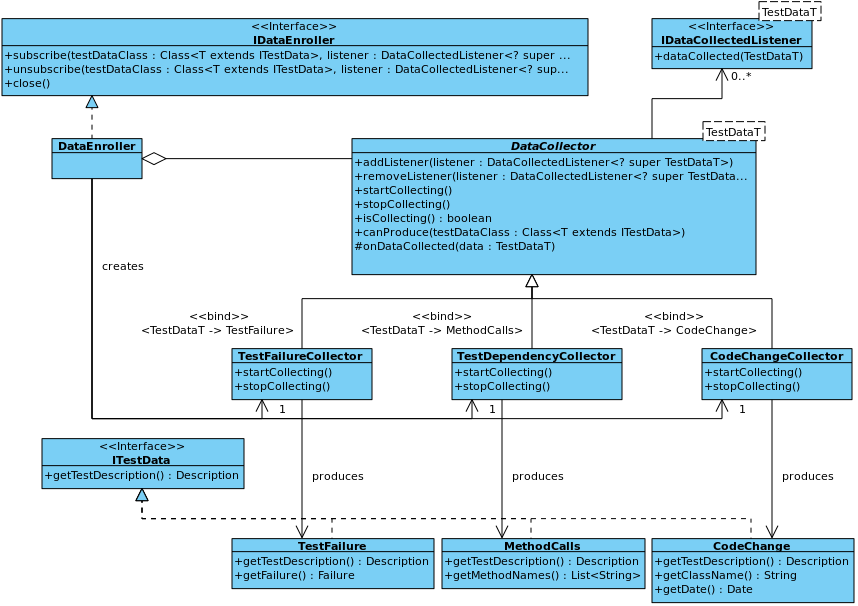
\includegraphics[width=0.8\textwidth]{DataCollectors}
    \caption{A class diagram of the package of data collectors}
	\label{fig:diagram:collectors}
\end{center}
\end{figure}

\subsubsection{Data collectors for specific types of data}

A concrete data collector is responsible for collecting only one kind of data.
Even though different data collectors can collect different kinds of data, their interface still remains the same, except for the type of the data itself. 
Moreover, an interested party is only interested in that kind of data, and nothing else.

An interested party does not want to check that the data item which it is being notified of, is actually of the type it is interested in.
This could be forced by a contract of the subscription, i.e. that the listener will only be notified of collected data of the type it is interested in.
However, the received data would still have to be cast to the correct type to actually be able to access the data and do something with it.

For these reasons, the \class{DataCollector} class is made generic in the type of data that it collects and notifies of.
It is thus actually declared as \class{DataCollector<T extends ITestData>}.
A concrete collector inherits from this class by filling in this generic type parameter \class{T}.
This type must extend \class{ITestData}, since collectors collect a subtype of \class{ITestData}, as was elaborated on in the previous subsection.

Concrete collectors are not generic themselves!
They have no reason to be, since they should know which data they collect.
For example, a \class{TestFailureCollector<MethodCalls>} would not make sense.
Therefore, the collectors are declared as follows, as is seen in figure \ref{fig:diagram:collectors}:
\begin{description}
\item[TestFailureCollector extends DataCollector<TestFailure>] \hfill \\ collects failures of tests
\item[TestDependencyCollector extends DataCollector<MethodCalls>] \hfill \\ collects the dependencies of a test, i.e. the methods that it calls
\item[CodeChangeCollector extends DataCollector<CodeChange>] \hfill \\ collects code changes that apply to tests
\end{description}

It follows that the \class{IDataCollectedListener} interface should also be generic (\class{IDataCollectedListener<T extends ITestData>}), since interested parties want to be notified only of a certain known concrete \class{ITestData} type.
Because it is generic, a concrete listener can fix the type of data it is interested in at compile time, rather than at run time. Casts are not necessary anymore and no additional checking of the validity of passed data items is required.

\subsubsection{Abstraction layer: IDataEnroller}

As was noted earlier, the design would benefit from an abstraction layer around the data collectors.

A first reason was that an interested party does not need to know which implementation of \class{DataCollector} is used to notify it of a collected data item. It does not even have to know of \class{DataCollector}s.

A second reason is that, however simple in interface, some data collectors may have an expensive mechanism to retrieve the data items in terms of resource usage.
These collectors should be shared.
For example, a \class{CodeChangeCollector} will have to watch directories and their subdirectories for file changes.
If multiple parties are interested in code changes, they should use the same underlying \class{CodeChangeCollector} (whether they know it or not).
The Observer pattern already allows the subscription of multiple listeners, but this does not mean that there's a good place by which the listeners can access them. 
Therefore, it is beneficial that an object exists which keeps track of all these collectors.

\class{IDataEnroller} is an interface for this new functionality imposed by the mentioned improvements.
Its only responsibility is to handle a subscription/unsubscription request for a listener for a specific kind of data.
Through classes that implement this interface, parties that are interested in a certain type of \class{ITestData} can register and unregister a listener.
As seen in the class diagram in figure \ref{fig:diagram:collectors}, a listener has to communicate the class of the \class{ITestData} it is interested in.

This abstraction does not communicate anything about \class{DataCollector}s to its users, so the first issue is solved.
The second one is not explicitly solved: sharing of data collectors is not required by this abstraction, since it doesn't even have to use \class{DataCollector}s.
However, the problem of sharing collectors is now moved to concrete \class{IDataEnroller}s.
They can decide for themselves what is best.

In our design, the concrete class \class{DataEnroller} is an implementation of the \class{IDataEnroller} interface.
This class will internally keep track of data collectors and will delegate a subscription or unsubscription request of listeners to a collector that supports the requested type of \class{ITestData}.
It is however not its responsibility to know which collector this is.
It is the collector itself that knows if it can produce a certain kind of \class{ITestData}, hence the method \method{canProduce(Class<T extends ITestData> testDataClass)} on the \class{DataCollector}.
Internally, this \class{DataEnroller} will ask each of its tracked \class{DataCollector}s if it can produce the requested type of data, until it finds one that can.
To this collector, it will delegate the subscription or unsubscription request.

If it does not find a collector that can produce the requested type of data, a \class{NoSuitableCollectorException} is thrown to indicate that the request can't be handled.

One thing that hasn't been discussed yet, is the creation of these collectors.
It certainly not is the responsibility of an interested party to create a collector. 
It is only interested in the data the collector produces.
This also isn't the responsibility of the \class{DataEnroller}, since it doesn't have to know how to create each possible collector.
However, due to a limited time, this creational aspect is not entirely implemented as it should be.
At this time, a static method \method{DataEnroller.createConfiguredDataEnroller} is present that creates a new \class{DataEnroller}, together with the collectors that have been implemented.
These created collectors are added to the new \class{DataEnroller} and the resulting instance is returned.

This creation, together with an example of a subscription of a listener, is illustrated in the sequence diagram in figure \ref{fig:sequence:subscribe-collector-listener}.

\begin{figure}[tbp]
\begin{center}
    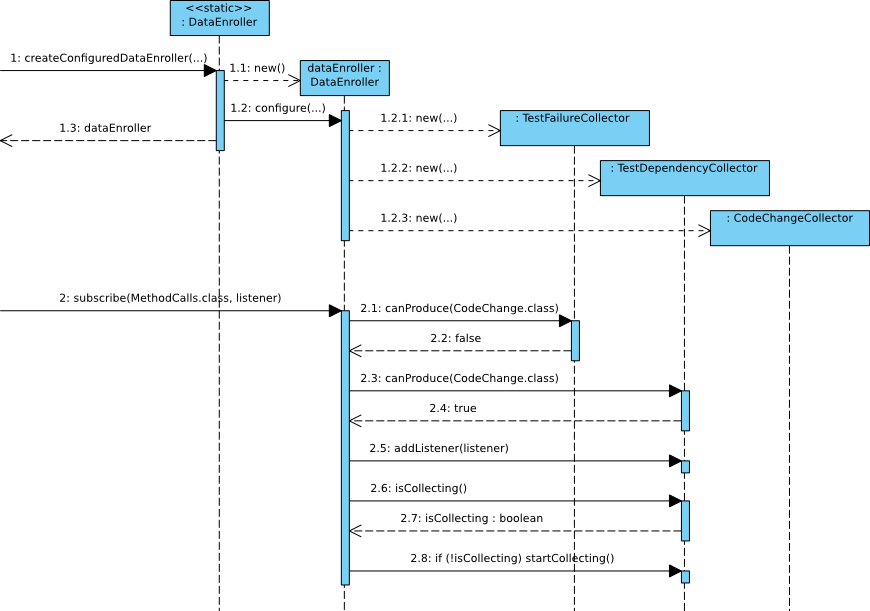
\includegraphics[width=0.9\textwidth]{SubscribeToDataCollector}
    \caption{A sequence diagram of the subscription of a listener to DataEnroller}
	\label{fig:sequence:subscribe-collector-listener}
\end{center}
\end{figure}

\subsubsection{Improvement: chain of factories}

Creating collectors is now done by \class{DataEnroller.createConfiguredDataEnroller}.
This is not an optimal solution, since this is not the responsibility of the \class{DataEnroller}.
This is now partially solved by putting the creational aspect inside a static method, that could easily be moved somewhere else.
However, better designs exist.

Now, the \method{createConfiguredDataEnroller} method must know how each collector has to be created.
It would be better to put the creation of each concrete \class{DataCollector} inside its own factory.
The \class{DataEnroller} would then only need to create the factories and ask the relevant factory for a collector.
Question remains how it can determine the relevant factory.
A solution would be to organize all these factories in a chain of responsibility.
Each factory would know itself for which concrete \class{ITestData} type it can create a collector.
By doing this, the \class{DataEnroller} can ask the chain to create a collector for a given class of \class{ITestData}.
The first factory in the chain would check if it can handle the request.
If not, it passes the request to the next factory.
If no link in the chain can handle the request, an exception would again be thrown.

\subsubsection{Data collector implementations}

Three types of collectors have been implemented, as can be seen in the class diagram in figure \ref{fig:diagram:collectors}.
They each are discussed in the following paragraphs.

\paragraph{TestFailureCollector} The \class{TestFailureCollector} extends \class{DataCollector<TestFailure>}.
As such, it notifies interested parties of \class{TestFailure}s it collects.
When this collector is created, a \class{RunNotificationSubscriber} object is passed to it, on which it will subscribe an internal subclass of the \junit \class{RunListener} class.
Subscribed \class{RunListener}s are notified by \junit when events in the flow of a testrun occur.
The event this collector needs is the event of a test failure.
When this event occurs, it will wrap the \junit failure inside a \class{TestFailure} instance, which this collector then passes to its subscribed interested parties.

\paragraph{TestDependencyCollector} The \class{TestDependencyCollector} extends \class{DataCollector<MethodCalls>}.
It will notify interested parties when it has collected a \class{MethodCalls} instance.
This \class{MethodCalls} object contains a list of methods that have been called by a test.
It is important that this is a list as opposed to another type of collection, since the order of executed methods may be important for some interested parties.
The executed methods are detected by using the provided \class{OSSRewriter} package.

Only the code under test should be looked at by this collector.
Therefore, this collector needs to know which classes belong to the code under test.
This is why the root directory of the code under test is passed when creating this collector.
It traverses this directory and keeps track of a list of all class files that it finds.
At this time, the collector knows which classes should be looked at for method calls, so it sets an exclusion filter on the \class{OSSRewriter}, so that other classes won't be rewritten by the \class{OSSRewriter} and only called methods in these classes are being notified of.

The actual notification of called methods is done by subscribing a \class{Monitor} to the \class{MonitorEntrypoint}, of which the \method{enterMethod(String methodName)} is called when a method of a rewritten class is entered. Note: these classes are classes of the \class{OSSRewriter} package, they are not written by us.

The only thing left to do, is determining which method call is executed by which test.
This is why this collector also needs to be passed a \class{RunNotificationSubscriber} during creation.
As with the \class{TestFailureCollector}, it will register an internal concrete \junit \class{RunListener}, which listens to the \emph{testStarted} and \emph{testFinished} event.
In response to the \emph{testStarted} event, this collector creates a new list of called methods (represented by strings).
The \emph{testStarted} event notifies of the end of a test, so this is the time that the collected method calls are complete. Consequently, a \class{MethodCalls} object is created with the collected list of called methods and interested parties are notified.
Of course, between the two events, the \method{enterMethod} method of the \class{Monitor} adds the method it is being notified of to the current \class{MethodCalls} object.

\subparagraph{Unsolved issue}

Tests running in parallel cause problems with the approach discussed here, since every \class{Monitor} receives notifications for every method that is called.
Thus, the \class{Monitor} can not easily make a distinction between methods executed by different tests.

One solution would be to check the stacktrace for each notification of a method execution. 
From this, the executing test could be determined.
However, it is suspected that this approach would be very expensive, since a stacktrace should be retrieved at each and every method call of the code under test.

Another solution would be to check in which thread a called method is run in.
This however is not always correct, since tests could cause other threads to be started.

Thus, it appears there is no clear solution for this problem.
Fortunately, the parallel scheduling of tests is only an experimental feature in \junit at this time, but in the future, this could become a problem.

\subparagraph{OSSRewriter remark}

The \class{OSSRewriter} package has a static interface.
Therefore, it is not easy to allow multiple parties to use this functionality.
The static interface forces one party to be responsible of setting up the \class{OSSRewriter}.
At this time, the \class{TestDependencyCollector} is the only class that uses it and only one instance is created of this collector.
Due to limited time, that instance was made responsible for enabling \class{OSSRewriter} and setting up the filter that excludes all code that is not code under test.
This should however be changed.
Ideally, a wrapper should be made around the \class{OSSRewriter} package that is responsible for enabling it.
This wrapper then could allow multiple parties to each register their own rewrite exclusion filter.

\paragraph{CodeChangeCollector}

The \class{CodeChangeCollector} extends \class{DataCollector<CodeChange>}.
It thus notifies its interested parties with \class{CodeChange} instances.
A \class{CodeChange} contains the name of the class name of a code change and the date that this change occurred.
The \class{CodeChangeCollector} needs to link a code change to a certain \class{Description}.
It however does not always know to which test this change corresponds, since it is not its responsibility to know which tests execute which code.
Therefore, it links a code change to the \junit \class{Description} of the root test suite class, since it is certain that the code change will apply to the root suite.

This collector uses a \class{WatchService} from the \class{java.nio.file} package.
The test directory and the directory of code under test is recursively registered with the \class{WatchService} for creation, deletion and modification events.
This means that when polling the \class{WatchService} for changes, all new, deleted and modified files and directories are picked up, in all subdirectories of the test directory and the directory of code under test.

It is obvious why these events need to be watched at for files.
When such an event occurs for a file, it will be checked if it is a *.class file.
If it is, a code change is detected: a new \class{CodeChange} is created and all interested parties (subscribed listeners) are notified.

It is however also important that these events need to be watched at for directories.
Each subdirectory in which the collector is interested, needs to be manually registered with the \class{WatchService}.
Therefore, it is important that when a directory changes its name, when it is deleted or when a new directory is created, these changes are detected, in response to which the \class{WatchService} needs to be updated with the changed interests.
Indeed, newly created directories or directories that have changed their name should be registered with the \class{WatchService}, otherwise, these changes are completely ignored after such an event.

This isn't even a rare event. For example, Eclipse removes all subdirectories in the binary folder when a project is cleaned and rebuilt. If these events were not taken into account, changes would not be detected anymore after one clean and rebuild operation, which completely undermines the objectives of the test daemon.

\subparagraph{Improvement} 

As was said, a code change is notified of by linking it to the root test suite \class{Description}.
While it can be argued that one is certain that a code change indeed applies to the root suite, this choice however is not great.
Two alternatives can be thought of.
The first would be that a data collector can also collect data items that are not tied to a \junit \class{Description}.
The responsibility of a data collector would then shift to the responsibility of collecting just \emph{a} data item, instead of a data item that applies to a certain \class{Description}.
However, a lot of classes notify others of new data, so they would al f



%-------DAEMON--------

\subsection{Daemon}
\label{subssec: deamon}

\class{Daemon} is responsible for repeated testing of a set of test classes. It monitors the directories of the tests and the nested classes. When a testrun is running it can message to the test-runs that a change in a file has occured. By handling the user input it will report the testrun that the active policy has changed or adding tests or removing tests . It will also receive the output of the testruns.  
% 
At the moment the \method{main} funtion is situated in the \class{Deamon}. This is not bounded with the \class{Deamon} but it was the most logical place to put the main. \class{Deamon} executes the testruns and if you would look for the \method{main()} you would search in the \class{Deamon}.

A difference between de \class{JUnitCore} and Deamon is that we could provide the \class{JUnitCore} with several suites, but to \class{Deamon} we can only give one \class{rootSuiteClass}. This \class{rootSuiteClass} consists of multiple suitesclasses.

Deamon functions as a Facade. It provides a simple interface. The Client will interact with the Deamon to the complex system that lays behind it.

%redenen voor een facade en waarom het een facade is.

% Facade ? 


%figuur oud klassendiagram
\begin{figure}[tbp]
\begin{center}
    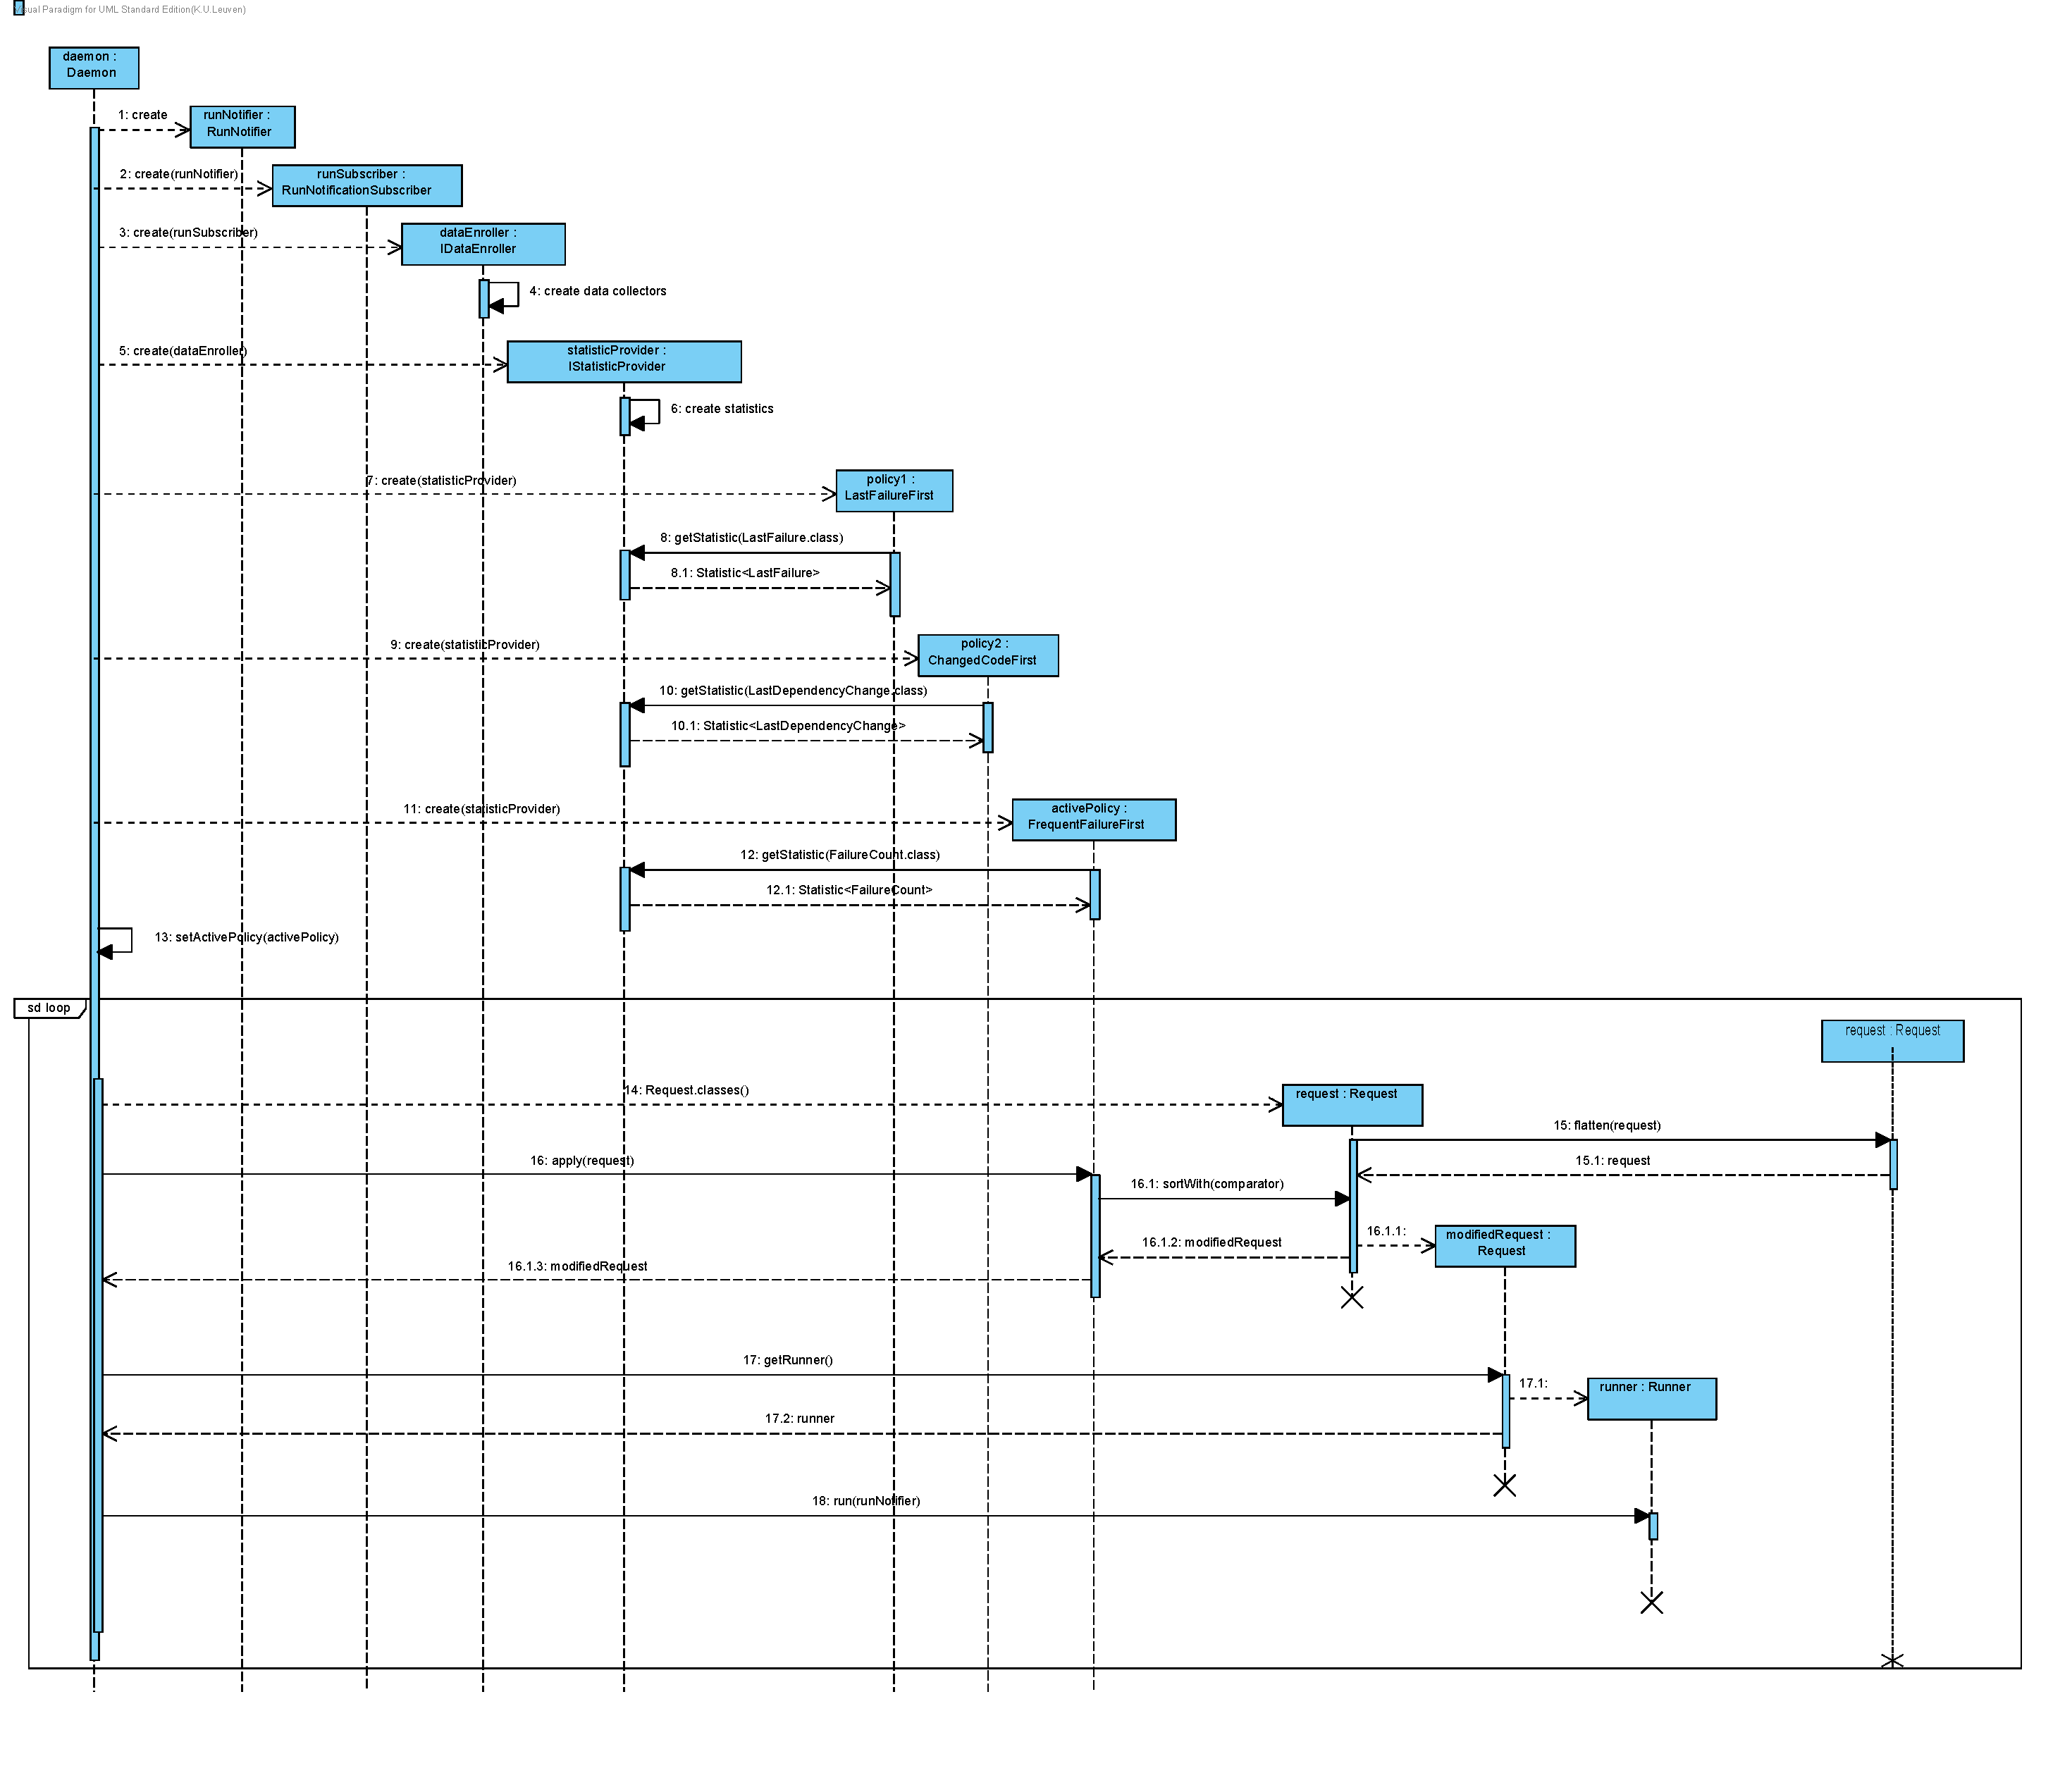
\includegraphics[width=0.8\textwidth]{RunATestrun}
    \caption{Sequence Diagram of a testrun}
	\label{fig:seq testrun}
\end{center}
\end{figure}


%-------STATISTICS-------

\subsection{Statistics}
\label{subssec: statistics}

%\begin{figure}[tbp]
%\begin{center}
%    \includegraphics[width=\textwidth]{Statistics}
%    \caption{Statistics Class Diagram}
%	\label{fig:statistics}
%\end{center}
%\end{figure}

The implemented \class{Statistic}'s will be discussed here in greater 
detail.
\begin{description}

\item [\class{FailureCountStatistic}] Collects the amount of times a test 
has failed until now.
A test is identified by its \class{Description}.
A \class{FailureCount} object is associated with this description,
representing the failure count.
When the \class{DataCollector} that this \class{Statistic} listens to
signals that a test has failed the counter inside the 
\class{FailureCount} is incremented.

\item [\class{MaxFailureCountStatistic}] This is a special kind of 
\class{FailureCountStatistic} where if the \class{Description} that it's
associated with is for multiple tests the highest failure count of its 
children is returned.

\item [\class{LastFailureStatistic}] This \class{Statistic} keeps the 
last time a test failed with a \class{LastFailureDate} object, which
wraps a \class{Date} object.

\item [\class{FailureTraceStatistic}] This \class{Statistic}, in contrast
with other \class{Statistic}'s, does not keep its state across multiple
test runs.
For each failing test in a test run a stack trace is collected. 
The last element in this stack trace is then the point of failure for 
this test.
A \class{String} that represents this point of failure is then wrapped
in a \class{FailureTrace} object.

\item [\class{LastDependencyChangeStatistic}] This \class{Statistic} uses
two different \class{DataCollector}'s to gather its statistics.
The first is a \class{TestDependencyCollector} which finds out which 
tests use which other classes by tracking the methods called by each
test.
The second is a \class{CodeChangeCollector} which reports changes to
class files in the project.
The \class{Statistic} then combines these data into 
\class{LastDependencyChange} objects.
These objects wrap the most recent date at which a dependency of the 
test it's associated with changed.

\end{description}

The statistics that are returned by \class{Statistic}'s implement the
\class{ITestStatistic} interface.
This interface specifies only the \method{getTestDescription()} method 
(perhaps not the most general name as the \class{Description} it returns
could be for a single test or a suite of tests).
Each implementing class then provides a getter method for the object it
wraps.

As with the \class{DataCollector}'s the abstract \class{Statistic} class
is generic in the type of \class{ITestStatistic} it returns but concrete
classes fill in this generic parameter to indicate which implementing
type of \class{ITestStatistic} they return, also to eliminate type 
checking that would be necessary in the \class{Policy}'s that receive
the collected \class{ITestStatistic}'s.

\class{Policy}'s that need the statistic value for a certain test call
the \method{getTestStatistic()} method on the \class{Statistic} object
they received from the \class{StatisticProvider}.
The \class{Statistic} does not (need to) know about what kind of objects
request this statistic data.
The clients of the \class{Statistic} class also don't need to be 
notified when the statistic value for a test changes as they may only
need a small subset of the available \class{ITestStatistic}'s and don't
need to be up-to-date on all of them all of the time.

The \method{getStatisticMethod()} is a template method.
It makes use of the abstract \method{composeTestStatistic()} method 
that differs in behaviour depending on the type of statistic that the
subclass collects.
The method can be used to calculate a compound statistic for a 
\class{Description} that is associated with a suite of tests.
The concrete implementation of this method then uses the statistics for
its children and produces some kind of summarized value from those (such
as a maximum, an average, ...)
In the case of \class{MaxFailureCountStatistic} the 
\method{composeTestStatistic} method takes the maximum of the failure
counts of the \class{Description}'s children.

The \class{StatisticProvider} is passed to a \class{Policy} on creation.
To get its needed \class{Statistic}(s) it passes the class of the 
\class{ITestStatistic}(s) it requires to the \class{StatisticProvider}
which then returns a \class{Statistic} that can produce this kind of
\class{ITestStatistic}.
To know which \class{Statistic} object to return the 
\class{StatisticProvider} keeps a \class{Set} of \class{Statistic}'s 
that are queried when a \class{Policy} requests a \class{Statistic}.
The \class{StatisticProvider} calls the \method{canSummarize()} method
on every \class{Statistic} in the set with the given 
\class{ITestStatistic} class and returns the first \class{Statistic}
for which this method returns \emph{true}.
In this way \class{Statistic}'s can be shared between \class{Policy}'s
which ensures consistency (if 2 different \class{Policy}'s request the
same statistic for the same test the response does not depend on when
the \class{Statistic} that that \class{Policy} uses was created).
It also makes switching \class{Policy}'s easier: when switching to 
another \class{Policy} that uses the same kind of 
\class{ITestStatisticData} statistics are already available.


%------POLICIES-------

\subsection{Policies}
\label{subssec: Policies}

Policies determine certain properties of a testrun, examples are
the order of tests and which tests are allowed to run (a filter).
The design of the policies follows the Strategy pattern.
Policies implement an interface \class{IPolicy} that specifies one method,
\method{apply}, which transforms a \class{Request}.
The abstract \class{SortingPolicy} defines the behaviour of sorting
policies with a template method, policies that extend this class have
only to implement a method \method{getComparator} that returns a 
\class{Comparator} that can compare two \class{Description}'s.
All implemented sorting policies make use of \class{Statistic}s to 
determine an order for tests, but this is not required.
At the moment, the following policies are supported: last failure first, 
frequent failure first, distinct failures first and changed code  first.
Each of these determines a different order that can be useful for
developers.
For example, tests that consistently order first under the frequent
failure first policy might indicate over-complicated or fragile code.

Originally we wanted to implement policies so they could be combined,
the composite pattern would be a good fit for this problem,
we decided against this because it was not required by the assignment.
However this would be a simple extension of the current design.
This combination of policies would be useful for example when you want
to use the frequent failure first policy but many tests fail with the
same frequency, you might want all tests with the same frequency ordered
by the last failure first policy.
Another use would be using a policy that filters all tests that haven't
failed yet together with a sorting policy.

\subsubsection{Frequent Failure First}

The frequent failure first policy is used to identify tests that fail
frequently.
This would be useful because a particular test failing often, may 
indicate that the code it tests is too complicated, so developers often 
break it or bugs don't get fixed (because people introduce separate 
handling of exceptions when finding a bug takes too much effort).
This policy makes use of \class{FailureCountStatistic}, tests with a 
higher number of failures go first, the order between tests with the same 
number of failures is undefined.
(\junit actually uses a stable sort, so this order would be the same as 
the original order, but this stability is not advertised in a contract 
and cannot be relied upon.)

\subsubsection{Last Failure First}

The last failure first policy prioritizes tests that have failed most 
recently.
The assumption being that tests that recently failed will most likely fail
again.
This policy uses \class{LastFailureStatistic} which provides the 
\class{Date} of the last failure of a test.
The order defined by this policy corresponds to the order of 
\class{Date}'s, most recent first.

\subsubsection{Distinct Failures First}

The distinct failures first policy specifies the most difficult 
ordering of tests.
Even at the level of single tests (i.e. a single method in a testcase)
the ordering is not trivial.
This is because it doesn't really matter if a certain test goes before 
another or not, what matters is that distinct failures are tested as 
quickly as possible.
For example if we have some tests (single methods) that failed in four
different ways, let's say failures A, B, C and D, then any test from 
one of these can go first, let's say a test from C goes first, then 
any test that failed on something different can go second, so now 
tests from A, B and D have priority over tests from C (A, B, D < C), 
when one test from every category has been executed, the order is again 
undefined.

This is a problem for the current implementation of \junit's 
\class{request} class.
This class uses a comparator to sort all of its tests, but as we can 
see, you can not define an order between any two tests because that 
order depends on what tests have already been chosen.
Because of this we decided that the distinct failures first policy would
determine a complete order for all it's tests.
This is a slight breach of the responsibilities of a sortingpolicy,
a policy is responsible for determining an order for tests,
however what tests it does this for should not be explicit in the 
policy.

When you need to sort not single tests but an entire suites of tests the 
ordering is even more difficult.
One suite may cover a part or everything of another suite, one suite 
may cover everything in two or more other suites but contain more tests 
without a failure and thus be less interesting to execute even if the 
suites it covers partly overlap.
This problem is similar to but not quite the same as the
"Set covering problem" (ref wikipedia), which is np-hard.
Because a complete and optimal solution is not critical and probably 
not worth the computational effort, we chose to implement a suboptimal 
solution. (i.e. a suite may go first if it contains a test that might 
have gone first if it was not in the suite. This suite could contain a 
method with a failure that has already been covered more times than any 
other but we don't check for this.)
We also decided to order single tests before suites for a specific 
failure because this increases the rate at which results for different 
failures can be shown, however between different failures a suite could 
go before a single test.

What follows is a description of the algorithm we implemented as a 
suboptimal solution to this problem.
(This algorithm determines an order and we will mention the term bucket,
however this algorithm has little to do with Bucket sort.)
When the DistinctFailureFirst policy is applied it first determines a 
(nearly) total order for all the descriptions in the request it is 
applied to.
The first step is to create a bucket for every failure that has 
happened during the previous testrun.
Then the bucket's are filled with every test and suite that fail on a 
particular failure.
A bucket contains every test(method) that fails on a certain failure 
and every suite that contains a test that fails on that failure and a 
counter for how many of it's descriptions have been selected.
When the bucket's have been created an iterative process of selection is
started:
\begin{enumerate}
	\item Choose a bucket with a minimal counter.
	\item Pick a description from this bucket.
	\item Remove this description from every bucket it appears in
    		(in case of a suite).
	\item Increment the counter for every bucket this description
    		appeared in.
	\item Record the description in a list that will contain a total 
    		order
            (only for failed tests, not for tests that did not fail)
			for all tests that failed.
	\item Repeat until all buckets are empty (actually empty buckets 
    		are removed, so until you run out of buckets).
\end{enumerate}
This leaves the order for tests without failures undetermined, but this policy is only interested in failures so this doesn't matter.
            
When using this policy's comparator the result is determined by the 
following rules:
If both descriptions appear in the list (total order) the order for the 
list applies.
If only one description appears in the list, it is ordered first.
If both description do not appear in the list then the order is not 
determined.

\subsubsection{Changed Code First}




%-------------KLASSENDIAGRAMMA------------------------------------------
%\subsection{Class diagrams} %-- Hier maken we geen aparte sectie van, en een volledig klassediagram zou veel groter moeten.
%# Akkoord wat het groter maken betreft. Het is misschien wel interessant om er een hoofding bij te zetten voor de duidelijkheid (eigenlijk vooral voor de index) maar het is niet de bedoeling dat er tekst bij staat. Of zie ik dat verkeerd.
%-- Ik zag het eerder als volgt. Mogelijks een volledig klassediagram in een appendix en voor de rest, waar nodig een gedetailleerd deeldiagram bij/in de tekst waar het bij hoort.
%# Mij goed, dan mag de subsectie weg.
%\label{ssec:Klassendiagramma}

%figuur nieuw klassendiagram
\begin{figure}[tbp]
\begin{center}
    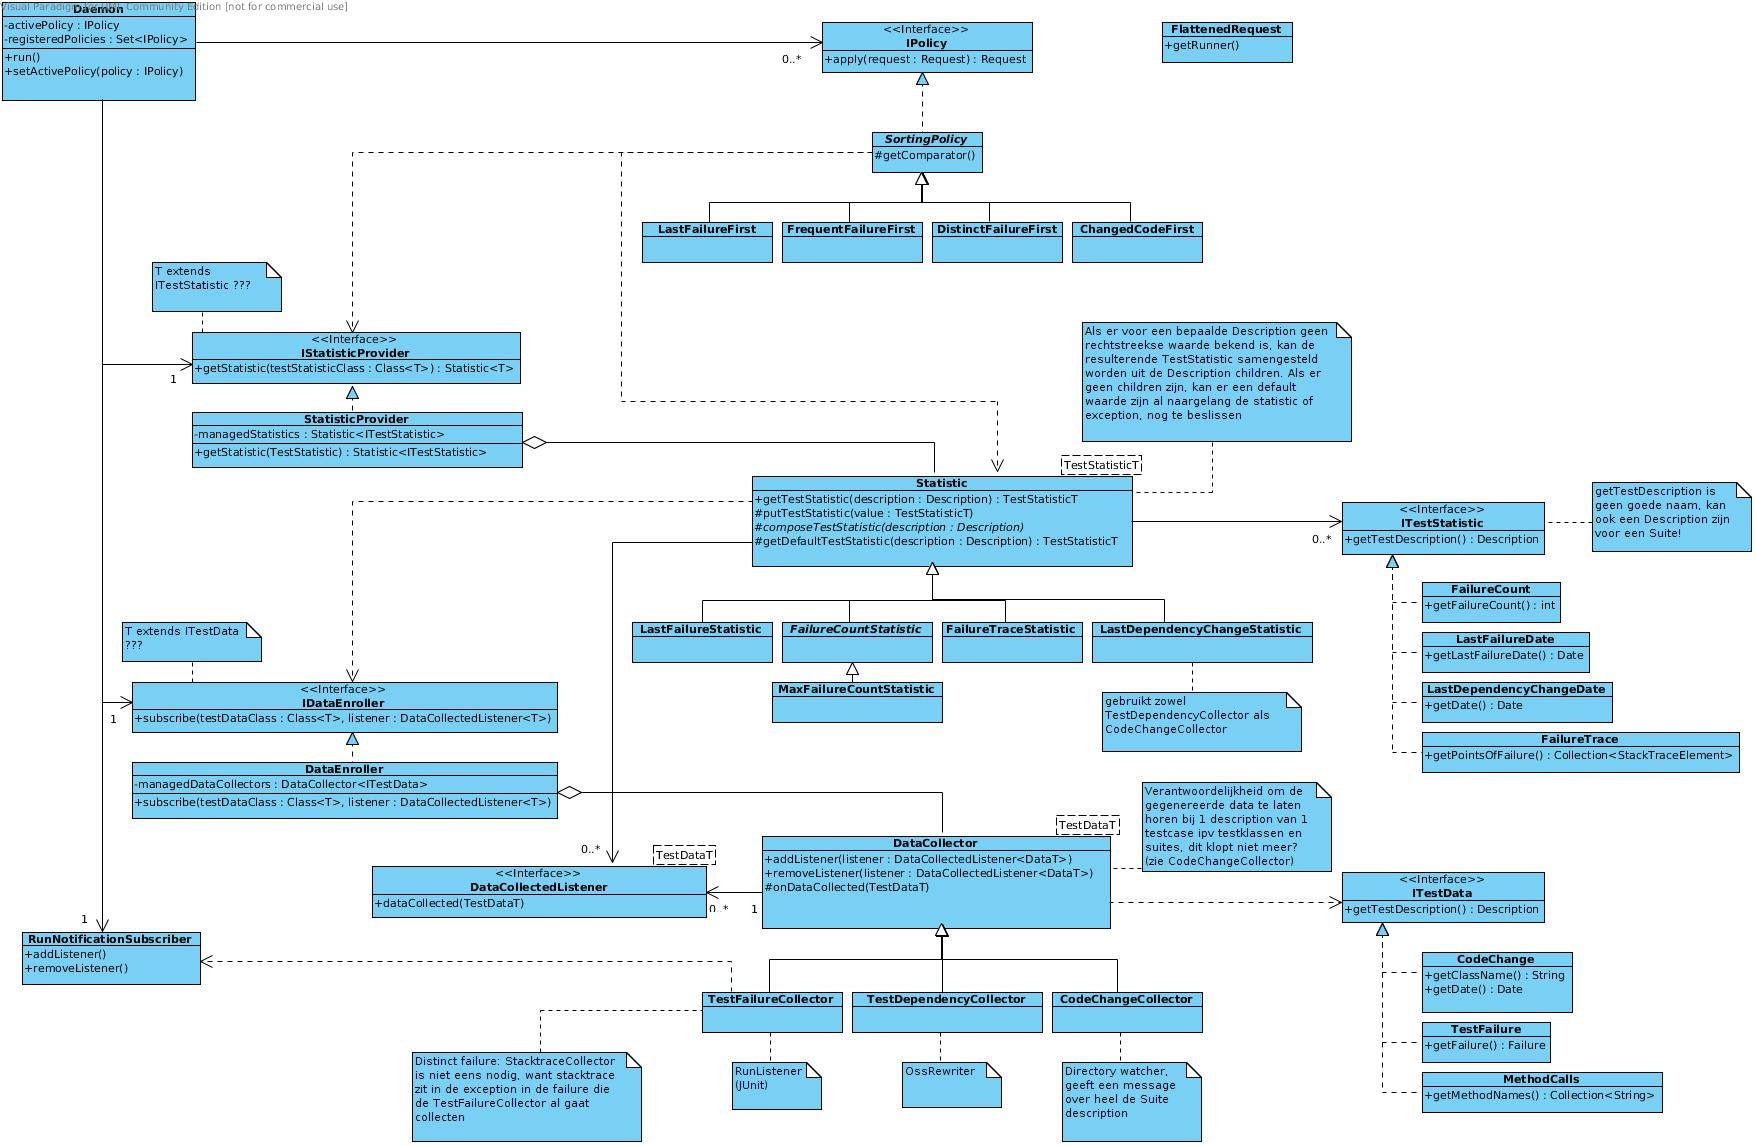
\includegraphics[width=0.8\textwidth]{klassendiagram3}
    \caption{Current classdiagram}
	\label{fig:kd-h}
\end{center}
\end{figure}



%-------------Interactie Diagrammas-------------------------------------
\subsection{Execution of Deamon}

The execution of the application starts with the \method{main()} method that is situated in the \class{Deamon}. The \method{main()} asks for three parameters. The first parameter is the suite of tests, the second is the directory were the code is that will be tested and the third parameter is the directory where the tests that will be executed are situated. If the parameters are correct, the deamon class will be created and given the three parameters and a console of his deamon will be started.  

When a \class{Deamon} is created there is also a \class{runNotifier} created. After that a \class{runNotificationSubscriber} is created with the \class{runNotifier}. Then a \class{DataEnroller} is created with the \class{runNotificationSubscriber} and the three parameters given with the \method{main()} function. The \class{DataEnroller} will create multiple data collectors. After that a \class{StatisticProvider} is created with the \class{DataEnroller} and the \class{RunNotificationSubscriber}. This \class{StatisticProvider} will create \class{Statistics}. At last the \class{FileChangedListener} is created that a \class{DataCollectorListener} is that will listen to  code changes.

After \Deamon is created the \class{ConsoleView} is started. The \class{ConsoleView} will ask the user to provide an active policy out of the list of registered policies. When the user has chosen the active policie, the \class{ConsoleView} will start the \Deamon. After that the user can still use commands throught the console by entering the right command. This command can incluse changing of policy, queue with a new testrun or quit. 

When \method{deamon.start()} is invoked in the \class{ConsoleView} it will subscribe to a \class{DataCollector} that collects data of code changes and it subscribes with the fileChangeListener that has been made previously. The \class{Semaphore} is set on one and the \method{startCore()} method is called. It will invoke the \class{Semaphore} to give a permit. In case of a grouped file changesm the system will stabilize first before really starting. After that the \method{doTestRun()} is invoked. This method will start the testrun.


The \method{doTestRun()} method is where it really starts. First a classLoader is created with the paths of the code directory and the test directory. It will then try to create a rootSuiteClass with the name that was provided with the main and the classLoader.
After that a \class{Request} is being made with the rootSuiteClass and the active policy. When the \class{Request} has been created, the runner is created of the \class{Request}. 

%The flow is as follows: first it will execute the main method. 

%-- Ho, stop, deze sectie moet daemon uitleggen, hier moogt ge nog niets zeggen over de execution van het programma dat is een grote subsectie binnen de sectie ontwerp.

%Three arguments are given with the execution. The first argument is the suite of tests, the second is the directory were the code is that will be tested and the third argument is the directory where the tests that will be executed are situated. After that it will start the \class{ConsoleView}. Through the \class{ConsoleView} the user can select which of the registered \class{Policy}'s will be used for the testrun. After the user selected a valid policy the \class{ConsoleView} will start the \class{Daemon} by calling the method start. If the \class{Daemon} is still running nothing this has no effect. If the \class{Daemon} is not yet running then a new thread will be created and it will subscribe itself to the \class{DataEnroller}. 
%TODO klopt dit?
%Then the \method{startCore()} method is called. Now the real execution of the Deamon is started
%# TODO



%-----------------------------------------------------------------------
%	TESTEN
%-----------------------------------------------------------------------
\section{Testing}
\label{ssec:testing}

For testing the application a two-fold approach was used: unit tests for
important classes and a dummy project to use the application on.
%# Voor zo ver ik gezien heb gebruiken we niet echt mocks, mocks verzamelen intern ook gegevens over de tests (zo kan een methode bijhouden hoe veel keer die is opgeroepen en zo'n dingen) en bestaan uit meer dan alleen maar stubs van methoden die opgeroepen worden in de tests.
%-- application vind ik eigenlijk niet zo'n goed woord voor wat we maken. En de two-fold is niet heel erg two-fold, we hebben geen twee manieren van testen, we hebben een nepproject om onze unit tests mee te kunnen doen.
%# Ah ik dacht dat het dummy project ook diende om de daemon zelf op te testen?
This dummy project includes some stub classes which contain methods that
exhibit behaviour that is interesting to test on.
For example there are classes that only include methods that throw 
exceptions.
There are also tests in this project that fail non-deterministically with 
different rates of failure to enable us to check if the sorting according 
to a test's failure rate happens correctly.



%-----------------------------------------------------------------------
%	PROJECT MANAGMENT
%-----------------------------------------------------------------------
\section{Project management}
\label{ssec:Projectmanag}
%taakverdeling elk lid en welke taak
%uren

We spent a lot of time on group discussions about the design of deamon and how we could implement everything. We did not always agree on everything and a lot of discussions followed. The first three weeks we spent a lot of time thinking about a good design for our program.\\ 
%-- Moet dit echt op deze manier? Het ligt toch nogal voor de hand dat we veel gediscussieerd/overlegd hebben als we er veel tijd in gestoken hebben. %% ja we zijn over de 40uur gegaan dat ze hadden gezegd en in verhouding hebben we veel meer gediscussieerd dan dat we geimplementeerd hebben

In the last half of week three and week four we started  implementing. One of the team members (Sophie) was on Athens that week and did not have time to help with the implementation. \\
%TODO tekst

The division of tasks was about the same for everybody. We worked in group most of the time. In figure \ref{tab:werkuren} the workhours per teammember can be seen for the different part of the assignment.

\comment{alles aanvullen!!}
\begin{table}[h!]
\begin{center}
    \begin{tabular}{ r | c  c  c  c  c  c}
     & Joren & Toon & Stef & Sophie \\ \hline
    Algemeen & 3u35 & 4u00 & 4u00 & 4u00\\
           Tools & 00u00 & 00u00 & 00u00 & 00u00 \\
        Analyse & 00u00 & 00u00 & 00u00 & 00u00 \\
        Design & 14u45 & 20u30 & 24u45 & 20u30 \\
        Implementation & 00u00 & 00u00 & 00u00 & 00u00\\
        Report & 9u00 & 9u00 & 9u00 & 9u00 \\
        Total & 29u30 & 29u30 & 31u15 & 27u30  
    \end{tabular}
    \caption{Overview of the workhours per subject}
    \label{tab:werkuren}
\end{center}
\end{table}

%TODO figuren updaten
\begin{figure}[h!]
        \centering
        \begin{subfigure}[hb]{0.20\textwidth}
                \centering
                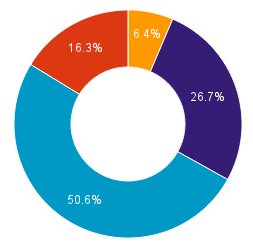
\includegraphics[width=\textwidth]{chart_2}
                \caption{Joren}
        \end{subfigure}%
        \begin{subfigure}[hb]{0.20\textwidth}
                \centering
                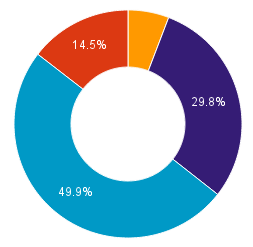
\includegraphics[width=\textwidth]{chart_3}
                \caption{Toon}
        \end{subfigure}%
        \begin{subfigure}[hb]{0.20\textwidth}
                \centering
                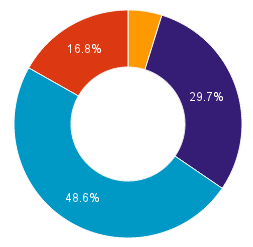
\includegraphics[width=\textwidth]{chart_4}
                \caption{Stef}
        \end{subfigure}%
        \begin{subfigure}[hb]{0.20\textwidth}
                \centering
                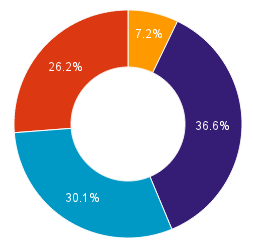
\includegraphics[width=\textwidth]{chart_5}
                \caption{Sophie}
        \end{subfigure}%
                \begin{subfigure}[hb]{0.20\textwidth}
                \centering
                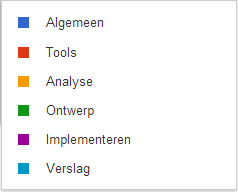
\includegraphics[width=\textwidth]{legende}
                \caption{Legend}
        \end{subfigure}%


 \caption{Overview of the division of tasks}
\label{fig:werkverdeling}
\end{figure}





%-----------------------------------------------------------------------
%	 CONCLUSIE en DISCUSSIE
%-----------------------------------------------------------------------
\section{Conclusion and discussion}
\label{ssec:conclusion}

% Een hoofdstuk met een discussie en conclusie waarin interessante ervaringen, problemen en
%andere opmerkingen omtrent het project worden beschreven


In the beginning of the design there were a lot of discussions about the overall implementation. We started with the Model-View-Controller pattern but it turned out that it was not that good. \\
%-- Ik snap niet waarom iedereen ineens zegt dat MVC niet goed is, we hebben dat gewoon niet gedaan omdat het niet nodig was, dat is iets heel anders.

In our first implementation we put every statistic and data in a big \class{StatisticPool} class. But after we spoke with the assistant we realized that it was a bad design because of the multiple dependencies with other classes and it was kind of god class in our design. \\

We spent a lot of time discussing the design of the \class{Daemon}. Sometimes we got stuck on a problem and we tried to find a solution but every solution had its own flaws. So we had to choose the solution with the least flaws. Not for every problem there is a pattern or design strategy. 
\\
%-- Ik zou liever niet zeggen dat er niet voor elk probleem een strategy is, strategies zijn normaal altijd toe te passen (scheiding van verantwoordelijkheden, low coupling, high cohesion, godclasses vermijden). Ik denk dat ge het hier hebt over onze oplossing met de "managers" enzo, en eigenlijk hebben we met die chain-of-responsibility daar wel een goede oplossing voor.







%-----------------------------------------------------------------------
%	GLOSSARY
%-----------------------------------------------------------------------

\section{Glossary}
\label{ssec:glossary}


\begin{description}
\item \gloss{CodeChangeCollector}\\
The class \class{CodeChangeCollector} collects dqtq from files that have been modified in the directory of tests and in the directory of code being tested. 
	

\item \gloss{Collector}\\
A collector collects information.

\item \gloss{Comparator}\\
A comparator imposes a total ordening on some collection of objects

\item \gloss{ConsoleView}\\
\class{ConsoleView} is the class that is the console view of the Deamon. It will give output to the user and the user can decide through the console view wich policy has to be set as active policy.

\item \gloss{DataCollector}\\
A \class{DataCollector} is responsible for collecting a certain type of information on tests. Any type is possible because the class had a generic type.

\item \gloss{DataEnroller}\\
\comment{TODO}

\item \gloss{Date}\\
The class \class{Date} represents a specific instant in time, with millisecond precision.

\item \gloss{Deamon} \\
	Deamon is responsible for executing the testruns. It can make use of different \class{Policy}'s to order the tests that need to be run.

\item \gloss{Description} \\ A \class{Description} describes a test which is to be run or has been run. 

\item \gloss{FailureCount} \\ 
\class{FailureCount} is a teststatistic that contains the number of fails for a test

\item \gloss{FailureCountStatistic}\\
A \class{FailureCountStatistic} is a \class{Statistic} that will collects the number of times a certain test has failed.

\item \gloss{FailureTraceStatistic}\\
A \class{FailureTraceStatistic} is a \class{Statistic} that stores \class{FailureTrace} instances for each test it has data for. When a new testrun starts, all stored \class{FailureTrace} instances are removed, since they don't have a use anymore.
	

\item \gloss{FlattenedRequest}\\
A \class{FLattenedRequest} flattens the test hierarchy of a given of a given \class{Request} by putting all the leaves at the same, single level. This can be useful to allow ordening of test methods across the levels and nodes of the original hierachy.

\item \gloss{filtering}\\
\comment{TODO}

\item \gloss{LastDependencyChange} \\
\class{LastDependencyChange} is a \class{teststatistic} that contains the date of the last change to a dependency for a test.

\class{LastDependencyChange} is a \class{Collector} that collects dependencies for tests and one that collects which files have changed.

\item \gloss{LastDependencyChangeStatistic} \\

The \class{LastDependencyChangeStatistic} is a \class{Statistic} that makes use of tzo \class{DataCollectors} to create \class{LastDependencyChange}'s. This \class{Statistic} will then combine that information to create \class{LastDependecyChange}'s.

\item \gloss{LastFailureDate} \\
\class{LastFailureDate} is a \class{teststatistic} that contains the date of the most recent failure of a test.

\item \gloss{LastFailureStatistic}\\
 The \class{LastFailureStatistic} is a \class{Statistic} that keeps the last time a test failed with a \class{LastFailureDate} object, which wraps a \class{Date} object.

\item \gloss{MaxCore} \\
\class{MaxCore} is a replacement for JUnitCore, which keeps track of runtime and failure history, and reorders tests to maximize the chances that a failing test occurs early in the test run.

\item \gloss{MaxFailureCountStatistic} \\
\comment{TODO}

\item \gloss{MethodRunner}\\
\comment{TODO}

\item \gloss{Policy} \\
A \class{Policy} imposes an order or filtering 

\item \gloss{Request} \\
A \class{Request} is an abstract description of tests to be run. 

\item \gloss{Runner} \\  A \gloss{Runner} is created for each class implied by the \gloss{Request}. The \class{Runner} returns a detailed \class{Description} which is a tree structure of the tests to be run.

\item \gloss{RunNotificationSubscriber} \\
\comment{TODO}


\item \gloss{RunNotifier} \\
\comment{TODO}

\item \gloss{SortingPolicy}\\
 A \class{SortingPolicy} determines an order for tests and suites. Examples of possible criteria for ordering: most frequent failures, shortest execution time.

\item \gloss{Statistic} \\
A \class{Statistic} listens to ITestData for tests and creates ITestStatistics for those tests.
%TODO misschien nog niet duidelijk zo

\item \gloss{StatisticProvider} \\
A \class{StatisticProvider} keeps the statistics and it will provide the \class{Policy} with the right \class{Statistic}.

\item \gloss{Testclass} \\
 A \class{TestClass} wraps a class to be run, providing method validation and annotation searching.

\item \gloss{TestDependencyCollector} \\
\class{TestDependencyCollector} is a \class{Collector} that collects all methods called by each test. This \class{Collector} assumes that the tests are run sequentially. If they are runned in parallel, the data collected by this \class{Collector} may be incorrect.


\item \gloss{Testrun} \\ 
	The run that executes the tests to be run.


\item \gloss{Unit Tests} \\
\comment{TODO}

 
\end{description}

%TODO hier kunnen we de patterns en strategies in vermelden
\newpage
\comment{Dit mogen we zeker niet vergeten aan te passen.}
\begin{flushleft}
\begin{thebibliography}{9}

\bibitem{TeamTreasure} 
\textit{Team Treasure Trek}
\begin{scriptsize}
geraadpleegd op 7/5/2013 via: \mbox{www.nintendo-europe.com/}
\end{scriptsize}

\bibitem{RabbitMQ}
\textit{RabbitMQ}
\begin{scriptsize}
geraadpleegd op 7/5/2013 via: \mbox{http://en.wikipedia.org/wiki/RabbitMQ}
\end{scriptsize}

\bibitem{mindstorms}
\textit{Lego Mindstorms}
\begin{scriptsize}
geraadpleegd op 7/5/2013 via: \mbox{www.lego.com} en \mbox{http://en.wikipedia.org/wiki/Lego\textendash Mindstorms}
\end{scriptsize}

\bibitem{leJOS}
\textit{leJOS}
\begin{scriptsize}
geraadpleegd op 7/5/2013 via: \mbox{http://lejos.sourceforge.net/}
\end{scriptsize}


\end{thebibliography}
\end{flushleft}

 

\end{document}